%!TEX TS-program = xelatex
%!TEX encoding = UTF-8 Unicode
% Awesome CV LaTeX Template for Cover Letter
%
% This template has been downloaded from:
% https://github.com/posquit0/Awesome-CV
%
% Authors:
% Claud D. Park <posquit0.bj@gmail.com>
% Lars Richter <mail@ayeks.de>
%
% Template license:
% CC BY-SA 4.0 (https://creativecommons.org/licenses/by-sa/4.0/)
%


%-------------------------------------------------------------------------------
% CONFIGURATIONS
%-------------------------------------------------------------------------------
\def\COLOR{00008b}
\def\HIGHLIGHT_TITLES{false}

% A4 paper size by default, use 'letterpaper' for US letter
\documentclass[11pt, a4paper]{awesome-cv}

% Configure page margins with geometry
\geometry{left=1.4cm, top=.8cm, right=1.4cm, bottom=1.8cm, footskip=.5cm}

% Specify the location of the included fonts
\fontdir[fonts/]

% Color for highlights
\definecolor{awesome}{HTML}{\COLOR}

% Colors for text
% Uncomment if you would like to specify your own color
%\definecolor{darktext}{HTML}{414141}
% \definecolor{text}{HTML}{333333}
%\definecolor{graytext}{HTML}{5D5D5D}
% \definecolor{lighttext}{HTML}{999999}

% Set false if you don't want to highlight section with awesome color
\setbool{acvSectionColorHighlight}{\HIGHLIGHT_TITLES}

% If you would like to change the social information separator from a pipe (|) to something else
\renewcommand{\acvHeaderSocialSep}{\quad\textbar\quad}


%-------------------------------------------------------------------------------
%	PERSONAL INFORMATION
%	Comment any of the lines below if they are not required
%-------------------------------------------------------------------------------
\def\FIRST_NAME{Gurdeep}
\def\LAST_NAME{Kumar}
\def\POSITION{Network Operations Engineer}
\def\ADRESS{}
\def\MOBILE{(+41) 0779932804}
\def\EMAIL{gurdipku91@gmail.com}
\def\GITHUB{hnnthecore}
\def\LINKEDIN{hnnthecore}
\def\HOMEPAGE{itswisskumar.ch}
\def\GITLAB{}
\def\SO_ID{}
\def\SO_NAME{}
\def\TWITTER{}
\def\SKYPE{}
\def\REDDIT_ID{}
\def\MEDIUM_ID{}
\def\GOOGLE_SCHOLAR_ID{}
\def\GOOGLE_SCHOLAR_NAME{}
\def\EXTRA_INFO{}
%\def\QUOTE{``You can' t judge a book by its cover"}
\def\QUOTE{``Quality is never an accident; it is always the result of intelligent effort."}
% Available options: circle|rectangle,edge/noedge,left/right

%\photo[right,rectangle,noedge]{./photo/photo.jpg}
\name{\FIRST_NAME}{\LAST_NAME}
\position{\POSITION}
%\address{\ADRESS}
\mobile{\MOBILE}
\email{\EMAIL}
\github{\GITHUB}
\linkedin{\LINKEDIN}
%\homepage{\HOMEPAGE}
% \gitlab{\GITLAB}
% \stackoverflow{\SO_ID}{\SO_NAME}
% \twitter{\TWITTER}
% \skype{\SKYPE}
% \reddit{\REDDIT_ID}
% \medium{\MEDIUM_ID}
% \googlescholar{\GOOGLE_SCHOLAR_ID}{\GOOGLE_SCHOLAR_NAME}
% \extrainfo{\EXTRA_INFO}

\quote{\QUOTE}


%-------------------------------------------------------------------------------
%	LETTER INFORMATION
%	All of the below lines must be filled out
%-------------------------------------------------------------------------------
% The company being applied to
%\recipient
%  {Swisscom}
%  {Alte Tiefenaustrasse 6\\
%  3048 Ittigen\\}
% The date on the letter, default is the date of compilation
\letterdate{\today}
% The title of the letter
\lettertitle{Bewerbung als Network Operations Engineer}
% How the letter is opened
\letteropening{}
% How the letter is closed
\letterclosing{Freundliche Grüsse,}
% Any enclosures with the letter
%\letterenclosure[Attached]{Curriculum Vitae}


%-------------------------------------------------------------------------------
\begin{document}

% Print the header with above personal informations
% Give optional argument to change alignment(C: center, L: left, R: right)
\makecvheader[R]

% Print the footer with 3 arguments(<left>, <center>, <right>)
% Leave any of these blank if they are not needed
\makecvfooter
  {\today}
  {\FIRST_NAME \LAST_NAME~~~·~~~Motivationsschreiben}
  {}

% Print the title with above letter informations
\makelettertitle

%-------------------------------------------------------------------------------
%	LETTER CONTENT
%-------------------------------------------------------------------------------
\begin{cvletter}
	

\lettersection{Über mich}

Ich bin eine zielstrebige und detailorientierte Person, die Wert auf Präzision legt. Meine Begeisterung für Technologie treibt mich dazu an, ständig Neues zu lernen, zu forschen und mich mit aktuellen Entwicklungen auseinanderzusetzen. Ich interessiere mich besonders dafür, wie Dinge funktionieren, und liebe es, Probleme zu lösen.

Mir ist es wichtig, nicht nur Neues zu lernen, sondern es auch wirklich zu verstehen. Ich bin überzeugt, dass kontinuierliches Lernen der Schlüssel zum Erfolg ist, deshalb halte ich mich immer über aktuelle Trends auf dem Laufenden. Diese Einstellung hilft mir, flexibel zu bleiben und mich weiterzuentwickeln. Zudem arbeite ich gerne mit anderen zusammen, um Wissen zu teilen und gemeinsam Neues zu schaffen. Mein Ziel ist es, meine technischen Fähigkeiten mit kreativen Ideen zu verbinden und an spannenden Projekten mitzuwirken.


\lettersection{Was qualifiziert mich als Network Operations Engineer?}
In den letzten Jahren habe ich mich intensiv mit Netzwerktechnik beschäftigt und grundlegende Kenntnisse über Protokolle wie TCP/IP, BGP, OSPF und HSRP aufgebaut. Zudem bin ich vertraut mit PPP, CDP, LLDP, STP, RSTP, EIGRP, PAT, NAT, HSRP, ACL und GRE sowie weiteren Netzwerkprotokollen. Darüber hinaus habe ich ein solides Verständnis für Netzwerkinfrastrukturen entwickelt.

Um meine Kenntnisse praktisch anzuwenden und zu vertiefen, baue ich aktuell mein eigenes Netzwerk-Labor mit physischer Hardware auf. Obwohl ich bereits praktische Erfahrung mit Netzwerksimulationen in **Cisco Packet Tracer und GNS3** gesammelt habe, war es mir wichtig, auch mit echter Hardware zu arbeiten. Dies ermöglicht es mir, nicht nur die theoretischen Konzepte besser zu verstehen, sondern auch reale Konfigurationen durchzuführen und praxisnah zu experimentieren.

Aktuell bereite ich mich auf die **SIZ-Zertifizierung** vor, für die ich in den nächsten Monaten meine Prüfungen ablegen werde. Da ich bereits intensiv für die **CCNA-Zertifizierung von Cisco** gelernt habe, aber die Prüfung verschoben habe, um genügend Zeit für die Vorbereitung auf die SIZ-Zertifizierung zu haben, plane ich, nach deren Abschluss das CCNA-Studium wieder intensiv aufzunehmen. Mein Ziel ist es, beide Zertifizierungen erfolgreich zu absolvieren.


Auch wenn ich noch keine umfangreiche Praxiserfahrung habe, bringe ich eine grosse Lernbereitschaft, Leidenschaft für Netzwerktechnologien und den Willen mit, mich kontinuierlich weiterzuentwickeln. 


\newpage % Nuova pagina

\lettersection{Mein Homelab}

Ich baue derzeit mein eigenes Networking-Labor auf, das es mir ermöglicht, verschiedene Netzwerktopologien und Protokolle praktisch zu testen. Derzeit arbeite ich an der Stromversorgung, da ich sicherstellen möchte, dass ich jeden einzelnen Router nach Bedarf ein- oder ausschalten kann, ohne alle Geräte gleichzeitig mit Strom zu versorgen. Sobald dieses System fertig ist, kann ich mein Homelab vollständig nutzen und noch flexibler mit meinen Tests arbeiten.

\begin{figure}[h!]
    \centering
    \begin{minipage}{0.48\textwidth} % Prima immagine
        \centering
        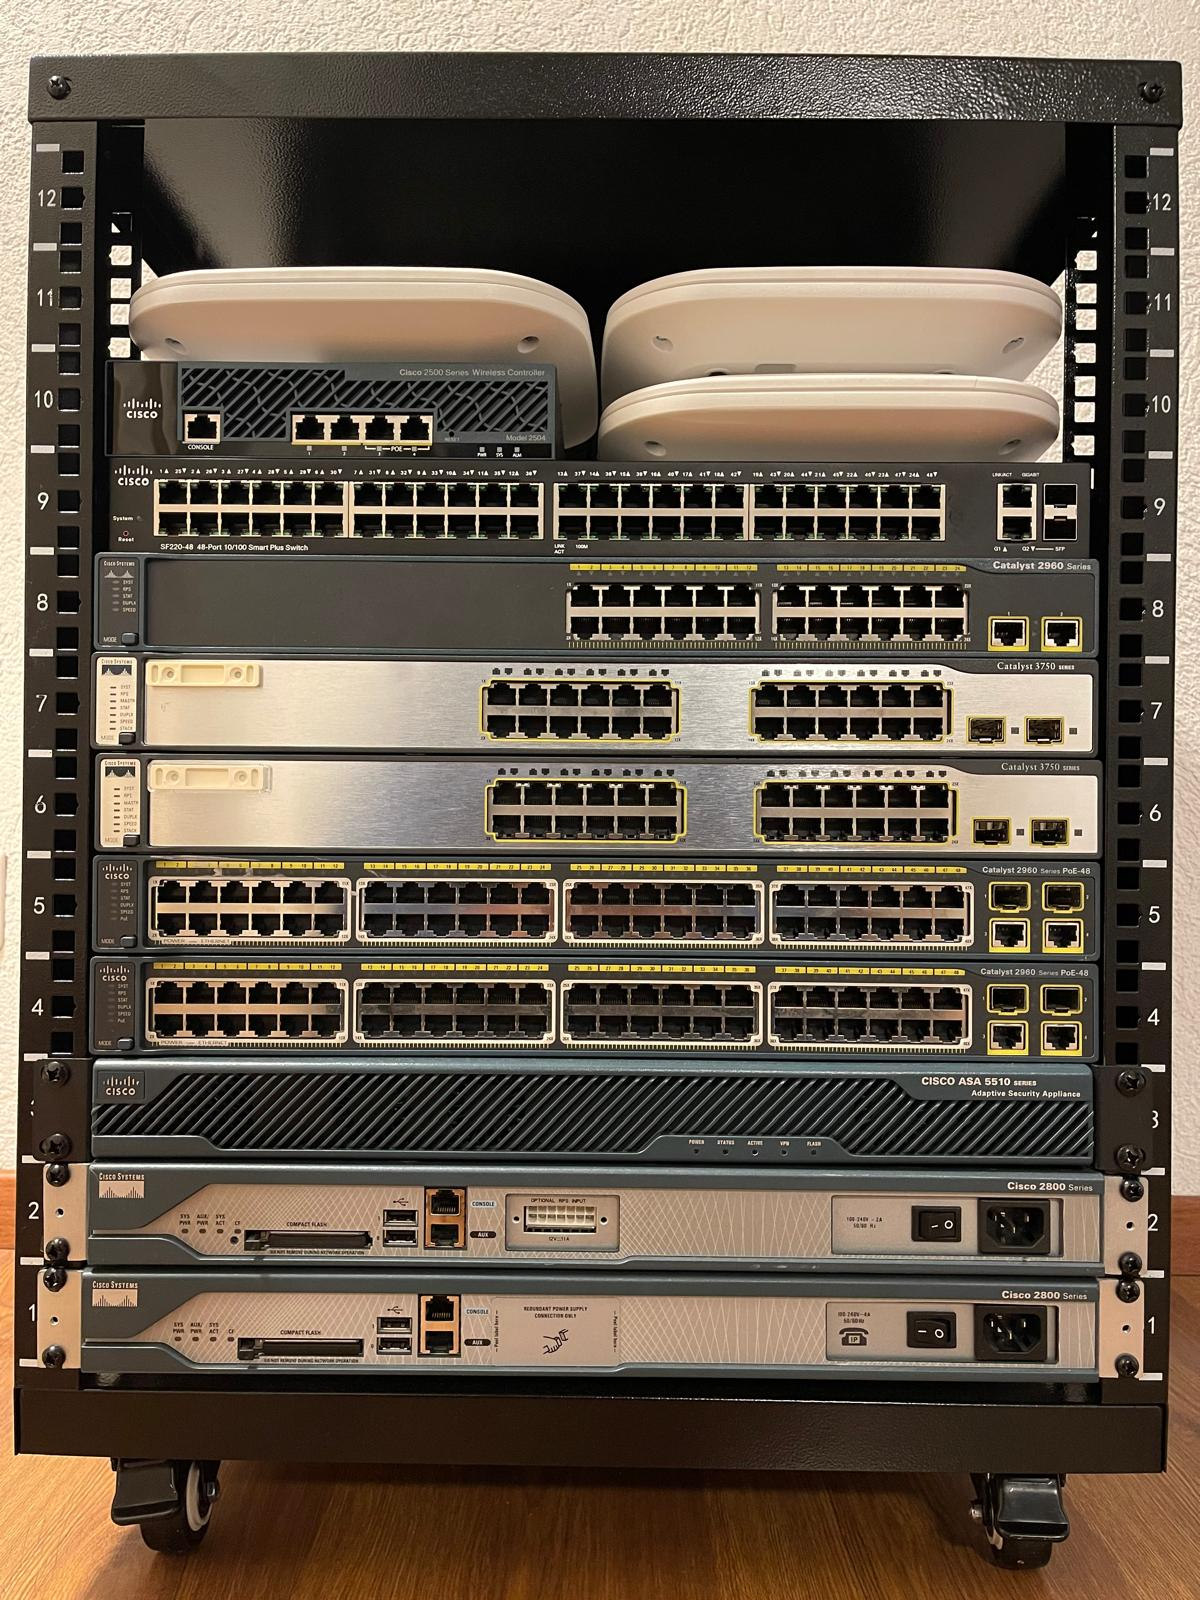
\includegraphics[width=\textwidth]{./foto_lab/lab_1.jpg}
        \caption{Vorderansicht meines Labs}
        \label{fig:lab1}
    \end{minipage}
    \hfill
    \begin{minipage}{0.48\textwidth} % Seconda immagine
        \centering
        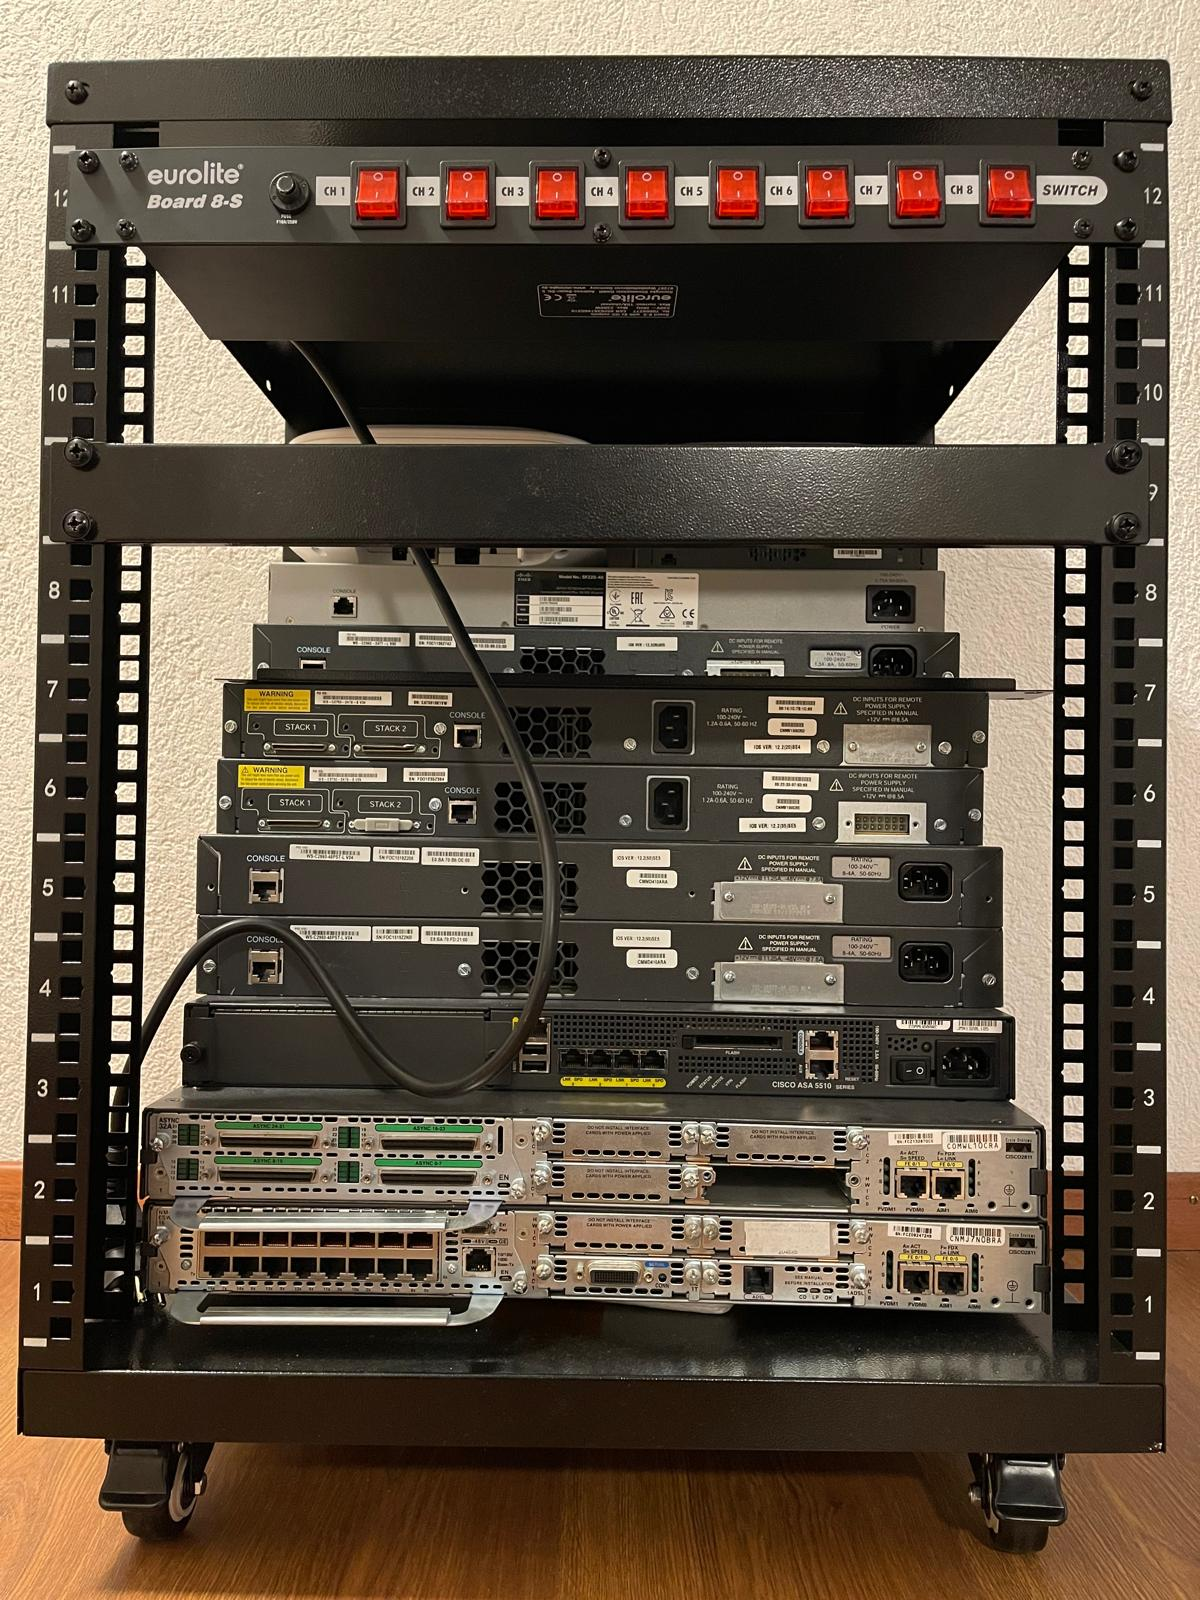
\includegraphics[width=\textwidth]{./foto_lab/lab3.jpg}
        \caption{Rückansicht meines Labs}
        \label{fig:lab2}
    \end{minipage}
\end{figure}

\vspace{0.5cm}

\textbf{In meinem Homelab befinden sich folgende Geräte:}
\begin{itemize}
    \item 2x Cisco 2800 Router
    \item 1x Cisco ASA 5510 Firewall
    \item 2x Cisco Catalyst 2960 Layer-2 Switches
    \item 2x Cisco Catalyst 3750 Layer-3 Switches
    \item 1x Cisco WLC 2500 Wireless Controller
    \item 3x Cisco Access Points
\end{itemize}


Dies ist mein persönliches Projekt im Bereich Networking, an dem ich aktuell arbeite. Zusätzlich habe ich noch weitere offene IT-Projekte, an denen ich abends nach der Arbeit und an den Wochenenden arbeite – zum Beispiel meine eigene Website, die ich nach meiner CCNA-Prüfung abschließen möchte. Ich würde gerne noch viel mehr über diese faszinierende Welt, insbesondere über Networking, sprechen, hoffe aber, dies in einem persönlichen Gespräch tun zu können.




\end{cvletter}


%-------------------------------------------------------------------------------
% Print the signature and enclosures with above letter informations
\makeletterclosing

\end{document}
